\section{Solving initial-value problems numerically}
Most differential equations can not be solved analytically, so we try to solve them numerically.

\subsection{Euler's method}
Suppose we have an initial-value problem:
\[\frac{dy}{dx}=f(x,y),\quad y(a)=y_0.\]
We want to find the solution $y(x)$ numerically on the interval $[a,b]$.

First we divide $[a,b]$ into $N$ equal subintervals by the points
\[a=x_0<x_1<x_2<\dots<x_k<\dots<x_N=b.\]

\begin{figure}[H]
\centering
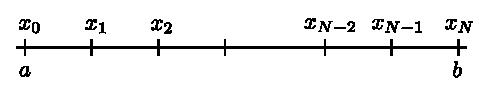
\includegraphics[scale=1.0]{img/subintervals-N}
\end{figure}

Similarly to when we looked at the trapezium method:
\[x_k=a+kh,\quad h=\frac{b-a}{N}\quad \text{(step size)},\quad k=0,1,\dots,N.\]

If $h$ is small, then the curve will be close to a straight line between $x_k$ and $x_{k+1}$.
The differential equation tells us that the gradient at $x_k$ is $f(x_k,y_k)$.
Therefore we approximate the curve between $x_k$ and $x_{k+1}$ by a straight line with gradient $f(x_k,y_k)$.

\begin{figure}[H]
\centering
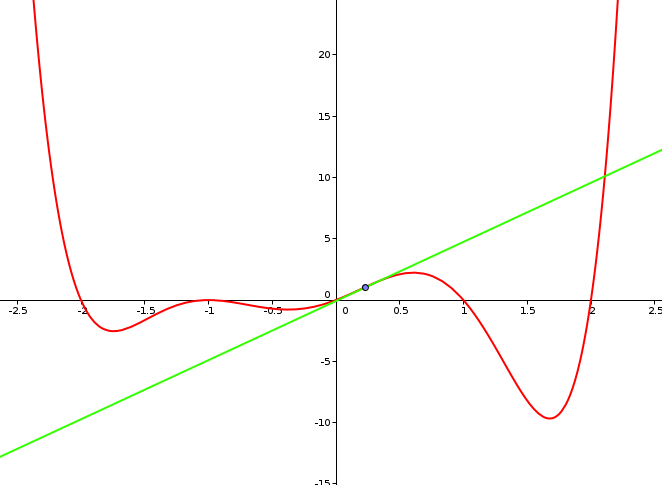
\includegraphics[width=.8\textwidth]{img/eulermethod}
\caption{Near the point marked, the curve (red) is closely approximated by the tangent (green).}
\end{figure}

This gives us the following approximation for $y_{k+1}$:

\[y_{k+1}=y_k + hf(x_k,y_k)\]

We know that $y_0=a$. We can then use this formula to approximate $y_1$, then use it again to find $y_2$, then $y_3$ and so on.
The method of approximating $y_k$ iteratively in this way is called \textbf{Euler's method}.

\begin{figure}[H]
\centering
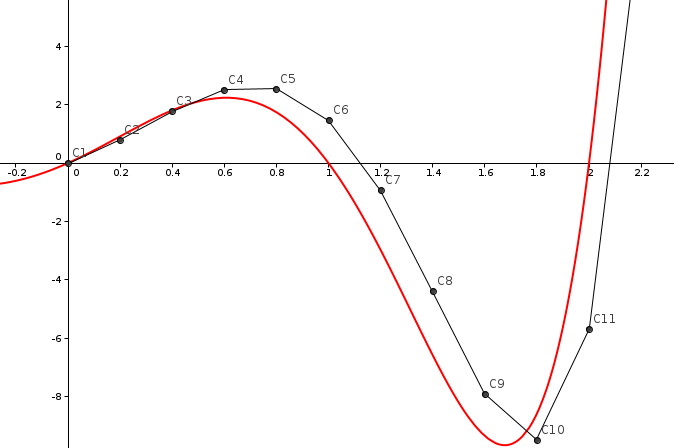
\includegraphics[width=.8\textwidth]{img/eulermethod2}
\caption{Using Euler's method to approximate a curve, starting at 0. at each point, a straight line is drawn with the gradient equal to that of the curve.}
\end{figure}

\begin{example}
Estimate $y(1)$, where $y(x)$ satisfies the initial-value problem: \[\frac{dy}{dx}=y,\quad y(0)=1.\] We 
know the exact solution is \[y(x)=e^x,\quad \implies\quad y(1)=e\approx2.71828.\]

\hrule
\vspace{2mm}

Now we apply Euler's method to the problem. We have 
\[f(x,y)=y.\]

First, we take $N=5$, then $h=(1-0)/5=0.2$. 

\begin{figure}[H]
\centering
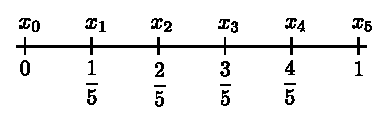
\includegraphics[scale=1.0]{img/subintervals-5}
\end{figure}
\begin{eqnarray*}
y_0 &=& y(0)=1 \\
y_1 &=& y_0+hf(x_0,y_0)=1+0.2\times1=1.2 \\
y_2 &=& y_1+hf(x_1,y_1)=1.2+0.2\times1.2=(1.2)^2 \\
y_3 &=& y_2 + hf(x_2,y_2)=y_2+hy_2=y_2(1+h)=(1.2)^2\times1.2=(1.2)^3 \\
y_4 &=& (1.2)^4 \\
y_5 &=& (1.2)^5\approx2.48832.
\end{eqnarray*}
Euler's method with 5 subintervals has given us the approximation \[y(1)\approx2.48832.\]
As we know the exact solution, we can look at the error:
\begin{align*}
\text{error}&=e-y_5\\&=2.71828-2.48832\\&=0.22996
\end{align*}

\hrule
\vspace{2mm}

Now, we double the number of subintervals: $N=10$, $h=0.1$ then we need 10 steps to reach $x_{10}=1$.
\[y_{10}=(1.1)^{10}\approx2.59374,\]
then we have
\[\text{error} = 2.71828-2.59374=0.12454.\]

\hrule
\vspace{2mm}

For $N=20$, $h=0.05$ and so
\[y_{20}=(1.05)^{20}\approx2.65330,\quad \text{error}=0.0650.\]

\hrule
\vspace{2mm}

For $N=40$, $h=0.025$ and so
\[y_{20}=(1.025)^{40}\approx2.68506,\quad \text{error}=0.0332.\]

\hrule
\vspace{2mm}

As we increase the number of intervals, the value becomes a better approximation.

\end{example}
